\chapter{Additional \DNLL scans for measurements}
\label{app:dnll_scans}


\begin{figure}[ht!]
\centering
\subfloat[\DNLL scan of \muV, profiling \muF and \mH]{
\label{fig:statandresults:mu_per_rv}
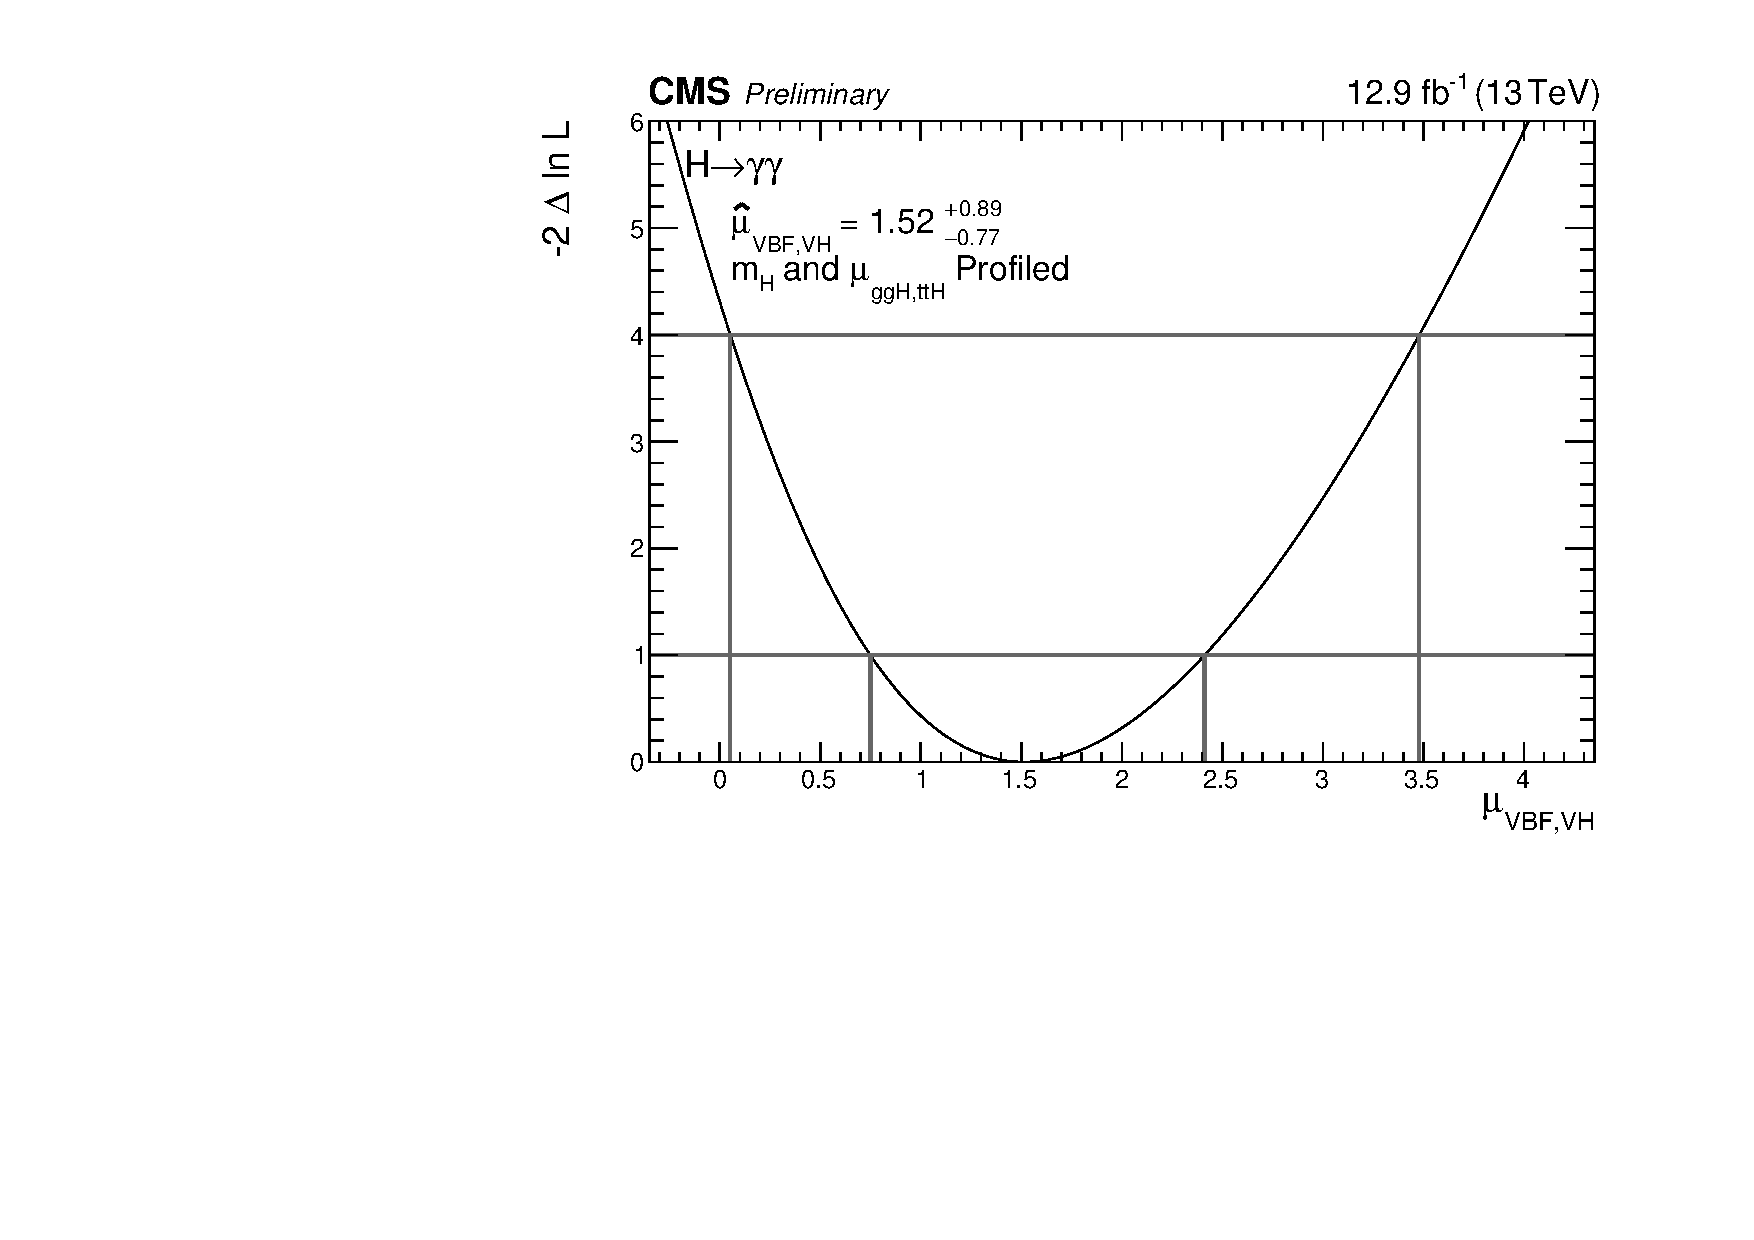
\includegraphics[width=0.8\textwidth]{statandresultsFigures/\whichFig/RVScanProfileMH.pdf}} \\
\subfloat[\DNLL scan of \muF, profiling \muV and \mH]{
\label{fig:statandresults:mu_per_rf}
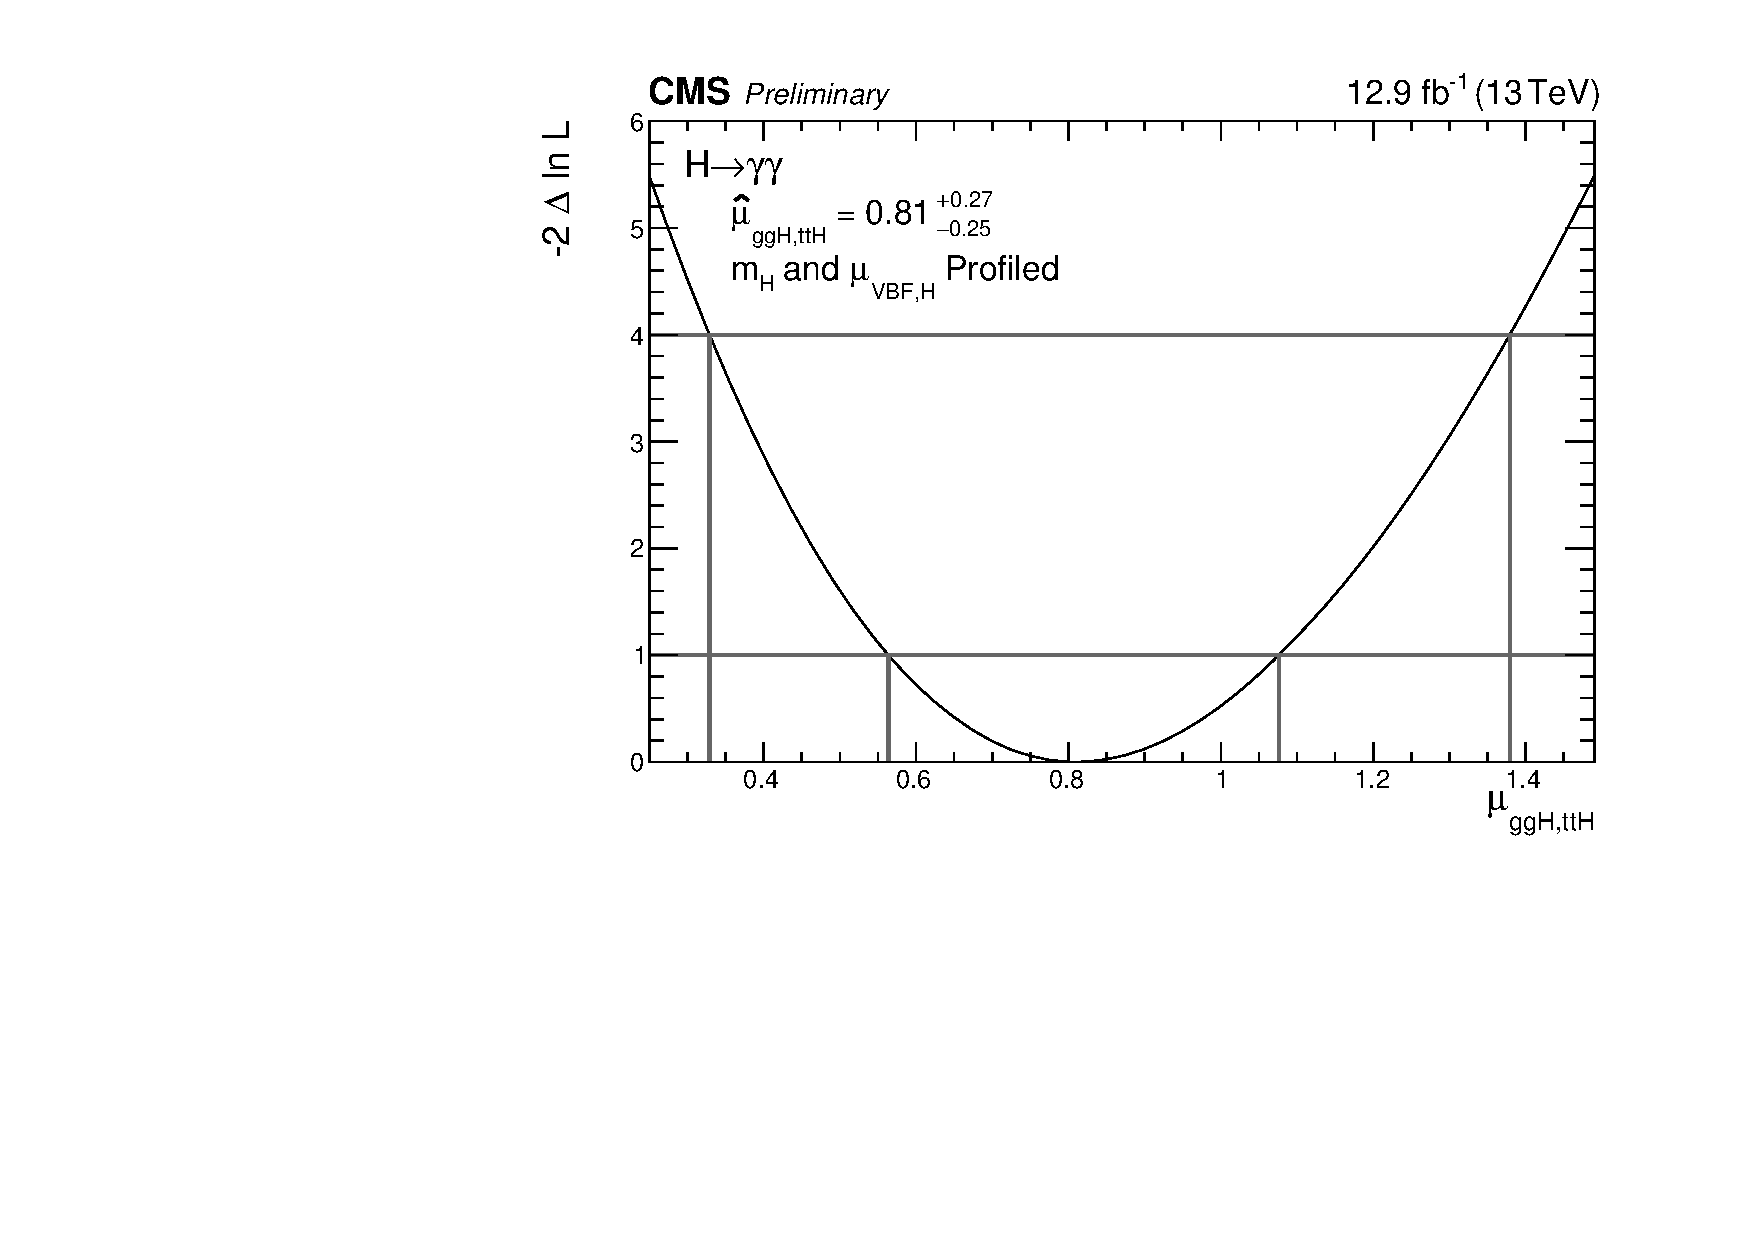
\includegraphics[width=0.8\textwidth]{statandresultsFigures/\whichFig/RFScanProfileMH.pdf}}
\caption{The result of performing \DNLL scans of \muV while profiling \muF (a) and vice versa (b). In both cases the mass of the Higgs boson is profiled in the fit. }
\label{fig:statandresults:mu_per_rv_and_rf}
\end{figure}

\begin{figure}[ht!]
\centering
\subfloat[\DNLL scan of \kV, profiling \kf and \mH]{
\label{fig:statandresults:kappa_per_v}
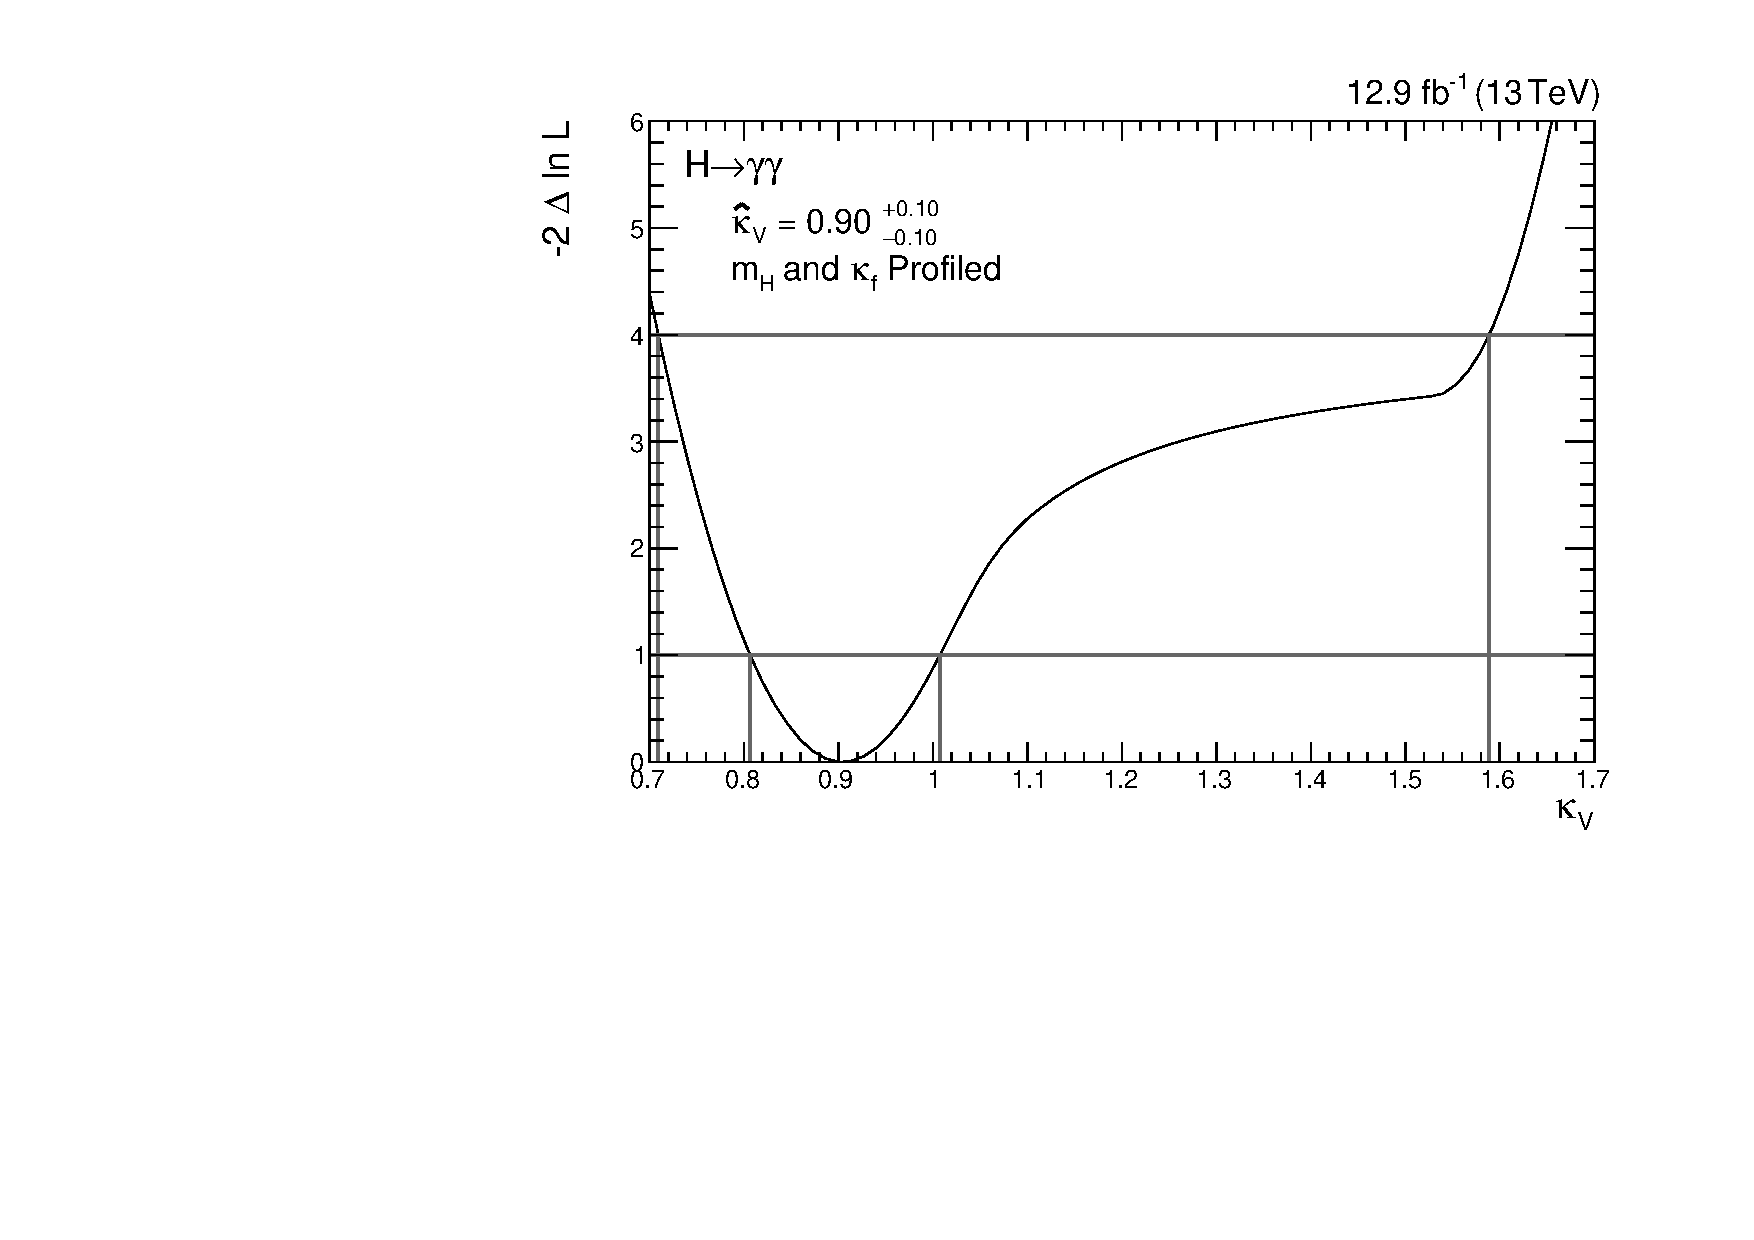
\includegraphics[width=0.8\textwidth]{statandresultsFigures/\whichFig/CVScanProfileMH.pdf}} \\
\subfloat[\DNLL scan of \kf, profiling \kV and \mH]{
\label{fig:statandresults:kappa_per_f}
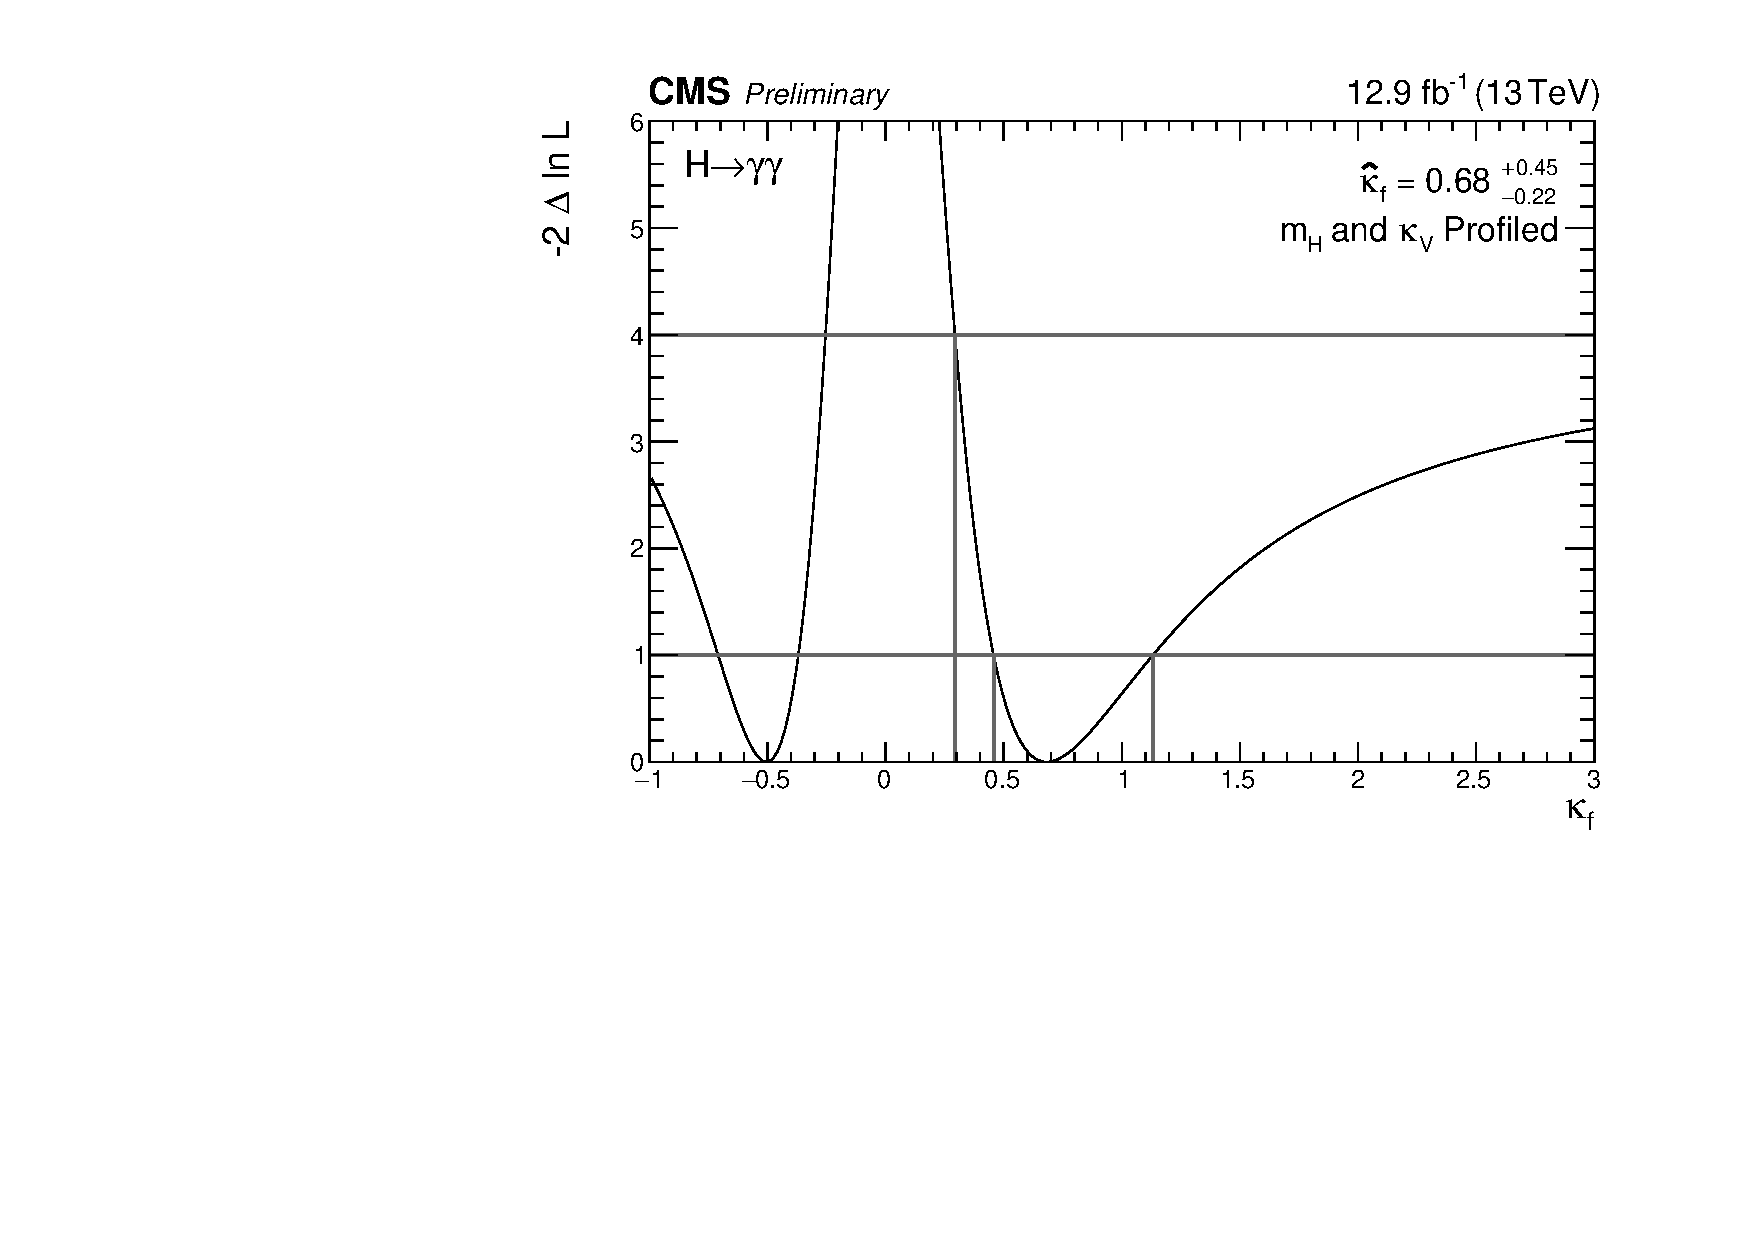
\includegraphics[width=0.8\textwidth]{statandresultsFigures/\whichFig/CFScanProfileMH.pdf}}
\caption{The result of performing \DNLL scans of \kV while profiling \kf (a) and vice versa (b). In both cases the mass of the Higgs boson is profiled in the fit. }
\label{fig:statandresults:kappa_per_v_and_f}
\end{figure}

\begin{figure}[ht!]
\centering
\subfloat[\DNLL scan of \kGlu, profiling \kPho and \mH]{
\label{fig:statandresults:kappa_per_glu}
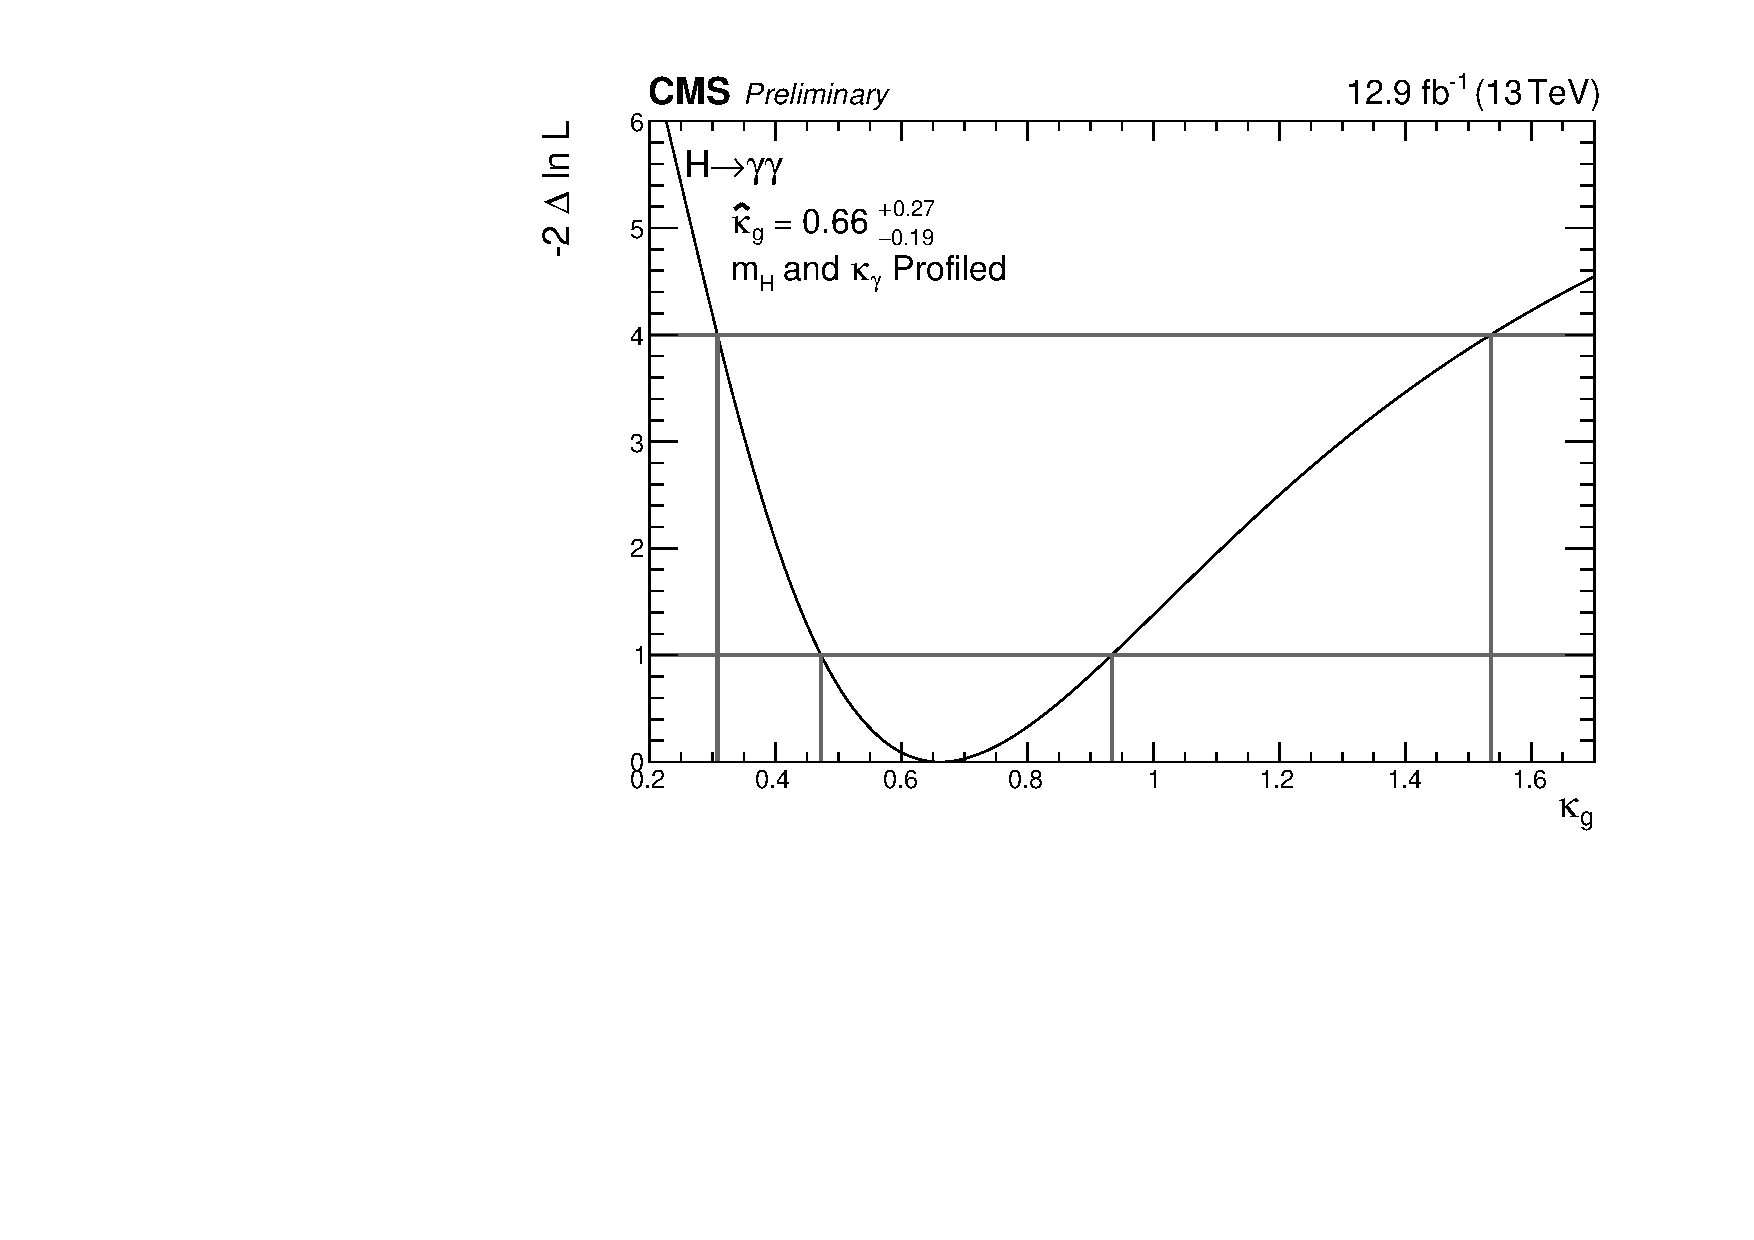
\includegraphics[width=0.8\textwidth]{statandresultsFigures/\whichFig/KGluScanProfileMH.pdf}} \\
\subfloat[\DNLL scan of \kPho, profiling \kGlu and \mH]{
\label{fig:statandresults:kappa_per_pho}
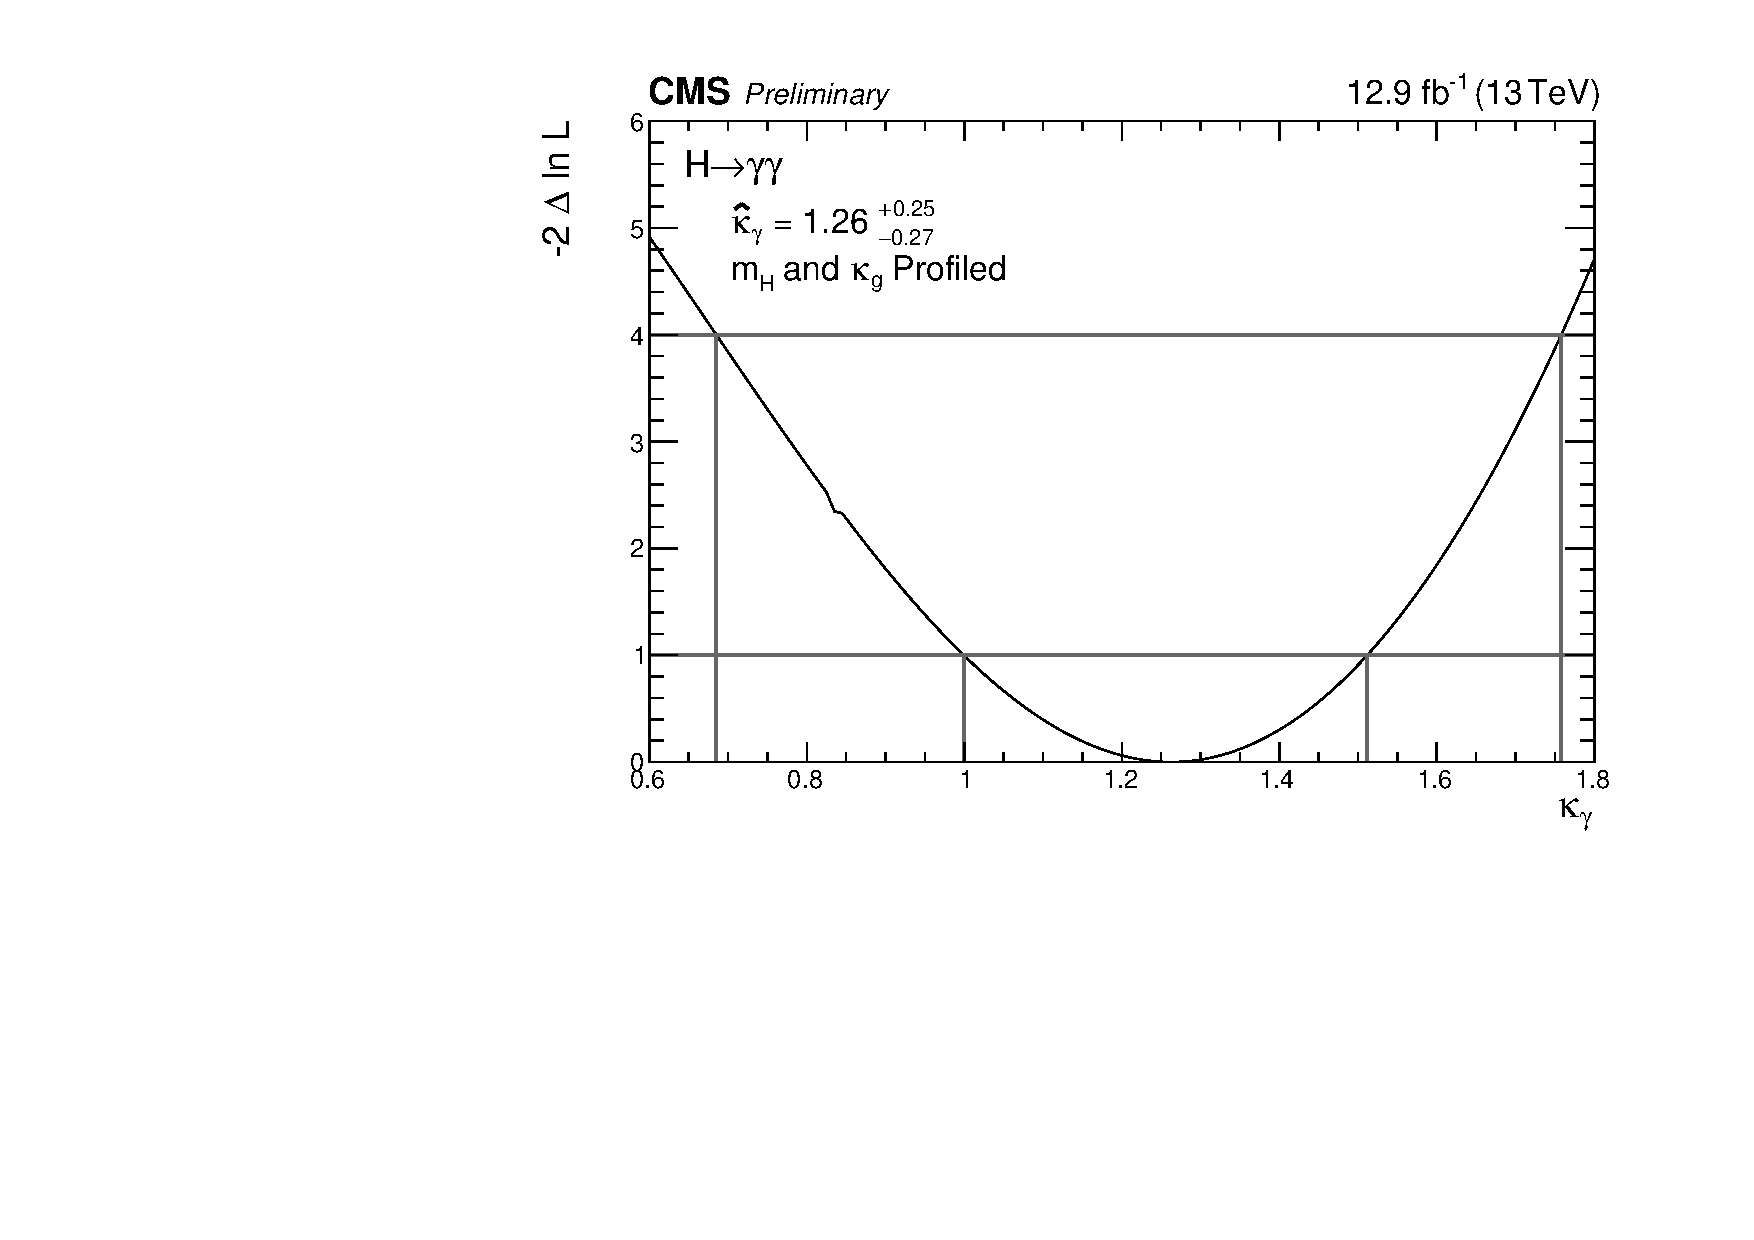
\includegraphics[width=0.8\textwidth]{statandresultsFigures/\whichFig/KGamScanProfileMH.pdf}}
\caption{The result of performing \DNLL scans of \kGlu while profiling \kPho (a) and vice versa (b). In both cases the mass of the Higgs boson is profiled in the fit. }
\label{fig:statandresults:kappa_per_g_and_g}
\end{figure}
